\section{Integralrechnung}
\todo{Intervalgrenzen tauschen $\rightarrow \cdot (-1)$}
\todo{Achtung bei Integral mit Grenzwerte welche Pol stellen beinhaltet!}

\subsection{Formeln}
\noindent Integral Ableitung mit Funktion-Limits: \[\left(\int_{a(x)}^{b(x)}f(t)dt\right)' = f(b(x))b'(x) - f(a(x))a'(x)\]
\noindent Integral Ungleichung:
\[\left|\int_{a}^{b}f(x)dx\right| \leq \int_{a}^{b}\left|f(x)\right|dx\]
\noindent RMS: 
\[\frac{1}{b-a}\int_{a}^{b}f(x)dx\]



\subsection{Methoden}
\[
\int(c_1f(x) + c_2g(x))dx \eqi c_1 \int f(x)dx + c_2 g(x) dx
\]

\textbf{Potenzregel} evt Partialbruchzerlegung!
\[
\int x^\alpha = \frac{x^{\alpha  + 1}}{\alpha + 1} + C
\]
\[
\int \frac{1}{x} = \ln\left|x\right| + C
\]

\textbf{Produktregel}
\[
\int f' \cdot g = f \cdot g - \int f \cdot g'
\]

\textbf{Allgemeine Substitution}
\todo{\[
	\int f(x) dx \eqi \int f(g(t)) \cdot g'(t)dt
	\]
Wobei $x=g(t)$ und $dx = g'(t)dt$
}

\textbf{Elementarsubst.}
\[
\int f(ax + b)dx = \frac{1}{a}F(ax+b)+C
\]

\textbf{Universalsubst. Trigo}\\
\todo{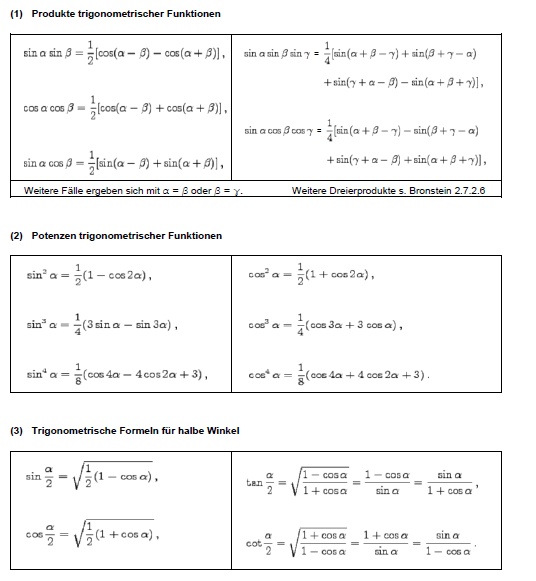
\includegraphics[width=0.7\linewidth]{Images/Trigo}}


\textbf{Potenzregel}\\
\textbf{Spezialfall Potenzregel $\alpha = -1$}\\
\textbf{Exponential allg.}\\
\textbf{Log-Integration}
\todo{woche 2}

\subsection{Majorante/Minorante}
\todo{Woche 3}
